\chapter{Methods}
\label{ch:methods}

\noindent In this chapter, the techniques adopted are explained from a theoretical perspective.
The chosen methods and related models are discussed to highlight the rationale behind their use to reach and evaluate the research goals defined in Chapter \ref{ch:introduction}.

The localisation system is defined by a sensor fusion approach to exploit the measurements available in a way that limits the different drawbacks of the sensors available.
The sensor fusion filter that will be used is a \gls{AEKF}, as it is a robust and adaptable.
It enables for the fast and reliable fusion of heterogeneous sensors in a way that will enable the \gls{ALM} to have a more accurate estimate of its pose.

The mapping approach is defined starting from the results of the localisation and exploiting the collision sensor installed in the \gls{ALM}.
Through the usage of these elements, a virtual boundary will be set and the presence of objects within it will be provided by the events fired by such a sensor.

Finally, the methodology adopted to evaluate the performances of these modules is defined.

The structure to provide localisation and mapping features is shown in Figure \ref{fig:structure}.


\begin{figure}[!ht]
	\begin{center}
		\begin{tikzpicture}[font=\small,thick]
			\node[draw, text centered, fill=white!30,
			align=center,
			minimum width=3cm,
			minimum height=1cm,
			] (block0) { Localisation };

			\node[draw, text centered, fill=white!30,rounded corners,
			above=2cm of block0,align=center,
			minimum width=2.5cm,
			minimum height=1cm,
			] (block01) { Kinematic\\Model };

			\node[draw,text centered,fill=white!30,rounded corners,
			left=of block0, align=center,
			minimum width=2cm,
			minimum height=1cm,
			] (block1) { \glspl{GNSS} };

			\node[draw,text centered,fill=white!30,rounded corners,
			above=0.5cm of block1, align=center,
			minimum width=2cm,
			minimum height=1cm,
			] (block2) { \gls{WO} };

			\node[draw,text centered,fill=white!30,rounded corners,
			left=0.5cm of block01,
			align=center,
			minimum width=2cm,
			minimum height=1cm,
			] (block3) { Control };

			\node[draw,text centered,fill=white!30,rounded corners,
			below=0.5cm of block1,
			align=center,
			minimum width=2cm,
			minimum height=1cm,
			] (block4) { \glspl{IMU} };

			\node[draw,text centered,fill=white!30,rounded corners,
			below=0.5cm of block4,
			align=center,
			minimum width=2cm,
			minimum height=1cm,
			] (block5) { \gls{VO} };

			\node[draw,text centered,fill=white!30,rounded corners,
			right=of block0,
			align=center,
			minimum width=2cm,
			minimum height=1cm,
			] (block6) { \textbf{Pose Estimation} };


			\node[draw,text centered,fill=white!30,
			right=of block6,
			align=center,
			minimum width=2cm,
			minimum height=1cm,
			] (block8) { Mapping };

			\node[draw,text centered,fill=white!30,rounded corners,
			above=of block8,
			align=center,
			minimum width=2cm,
			minimum height=1cm,
			] (block7) { Collision };

			\node[draw,text centered,fill=white!30,rounded corners,
			below=of block8,
			align=center,
			minimum width=2cm,
			minimum height=1cm,
			] (block9) { \textbf{Occupancy Grid} };

			% Arrows
			\draw[-latex] (block1) edge (block0);% node [above, fill=white] {Label Text};
			\draw[-latex] (block01) edge (block0);
			\draw[-latex] (block2) edge (block0);
			\draw[-latex] (block3) edge (block0);
			\draw[-latex] (block4) edge (block0);
			\draw[-latex] (block5) edge (block0);
			\draw[-latex] (block0) edge (block6);
			\draw[-latex] (block6) edge (block8);
			\draw[-latex] (block7) edge (block8);
			\draw[-latex] (block8) edge (block9);

		\end{tikzpicture}
		\caption[Caption]{Structure of the Solution\centering}
		\label{fig:structure}
	\end{center}
\end{figure}

\noindent
RISE AB, in collaboration with Husqvarna AB, is interested in the research and development of a refined approach to improve the performance of the \gls{ALM}, thus allowing for the development of more features.
The system will be built upon the \Gls{HRP}~\cite{HRP}, a \Gls{ROS} enabled Husqvarna Automower 450X with additional sensors assembled upon it, as shown in Figure \ref{fig:HardwareSetup}.
It has been improved by a former thesis student~\cite{HRPTianze} and it is now equipped with additional two \Glspl{IMU}, two \Gls{GNSS} signal receivers, and a \Gls{RGBD} camera.

\begin{figure}[!ht]
	\begin{center}
		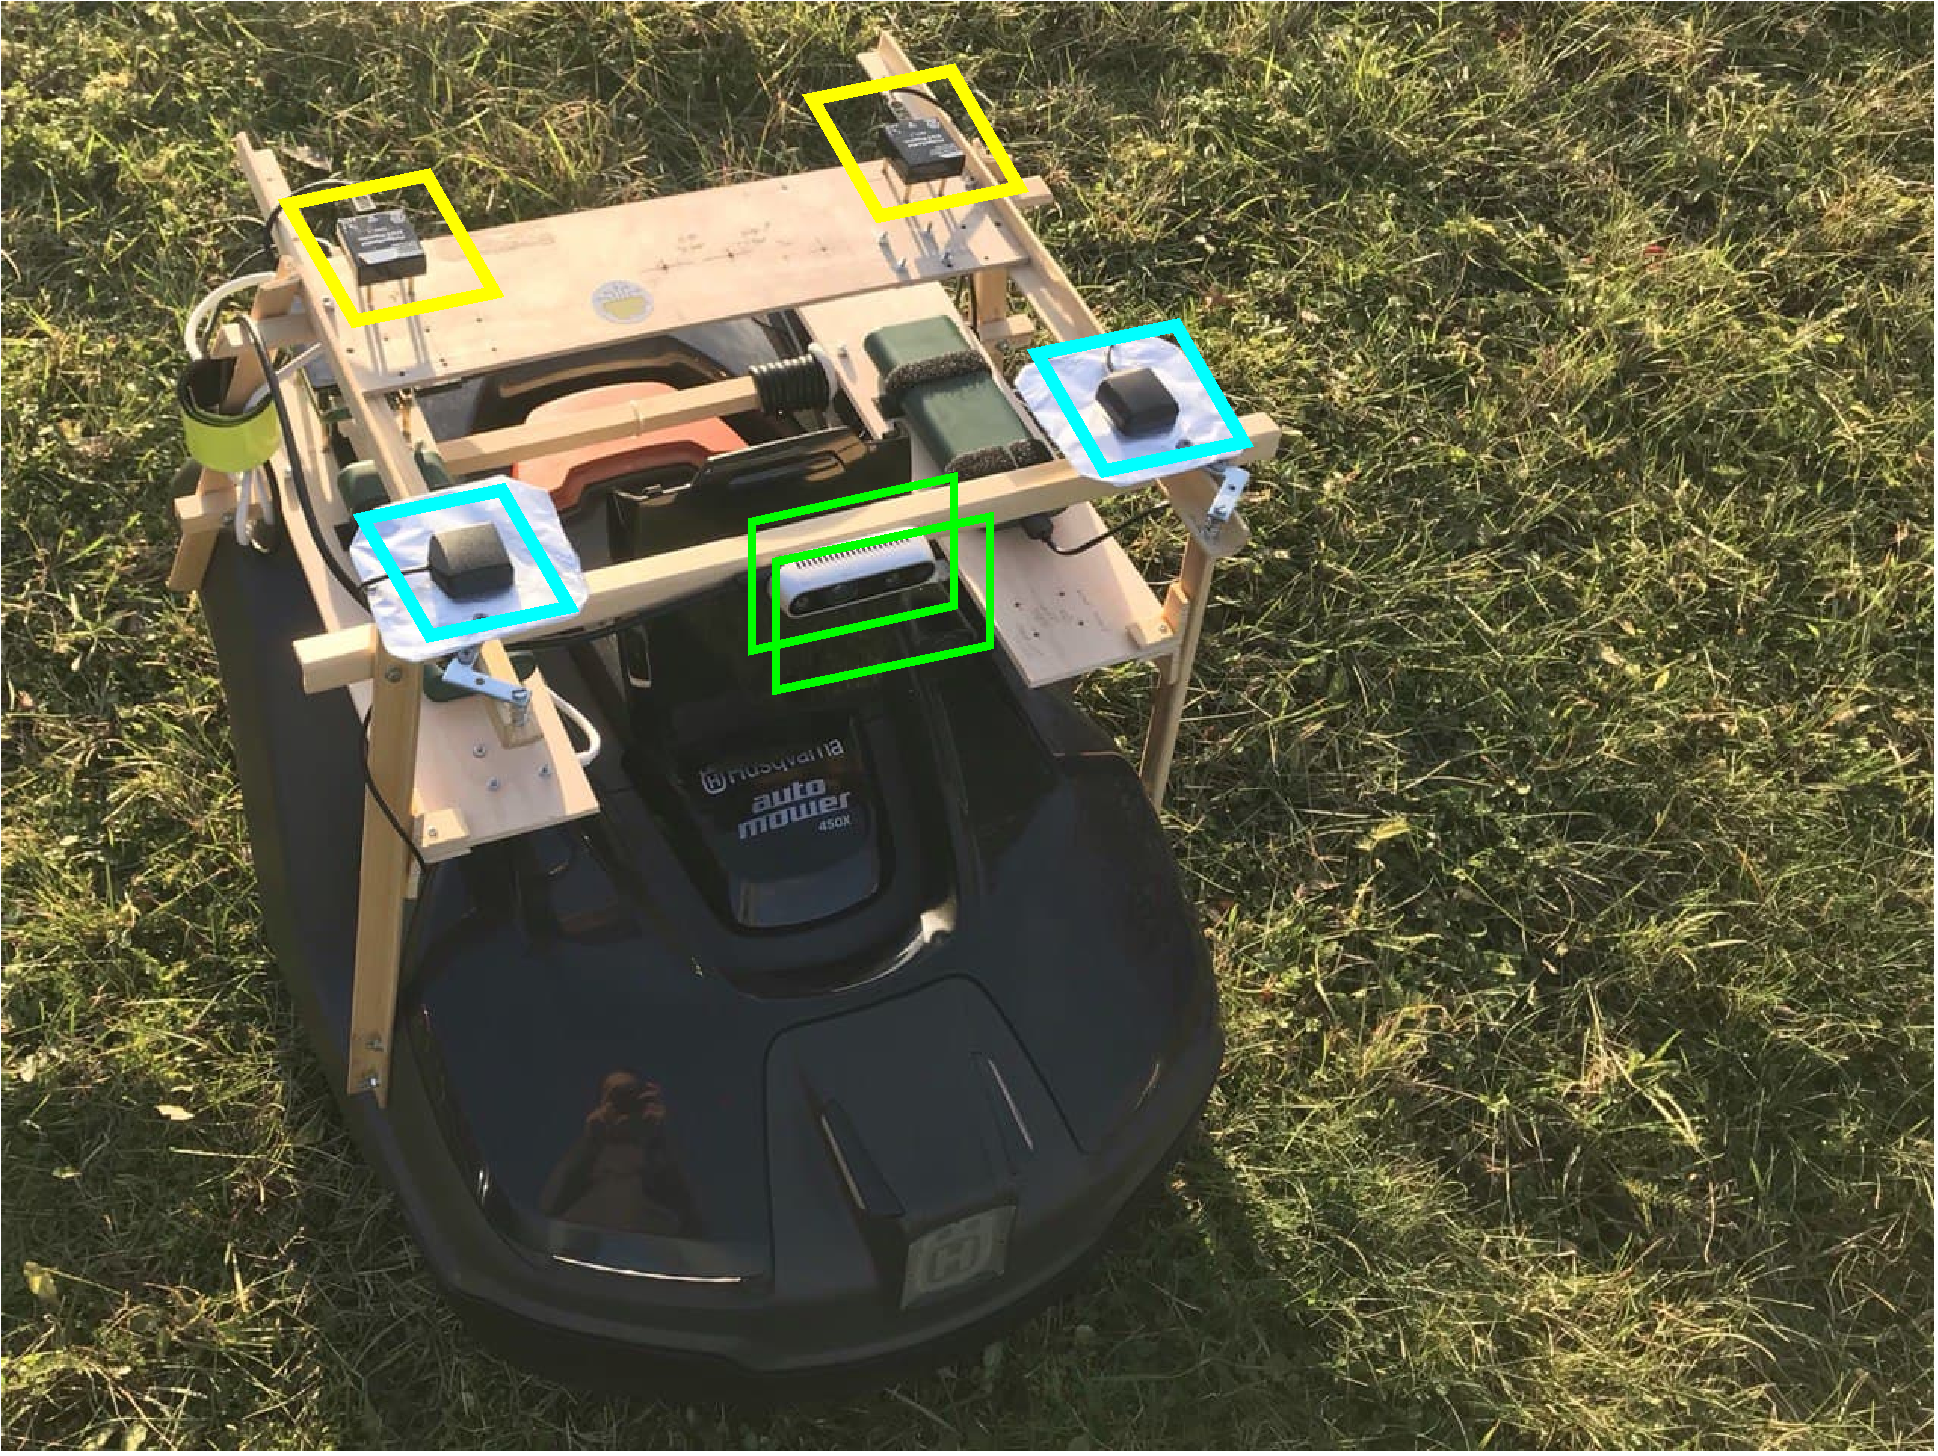
\includegraphics[width=1.0\textwidth]{Images/1-Introduction/projectTheme.pdf}
		\caption{
			\gls{ALM} Model with focus on additional sensors:\\
			\glspl{IMU} [yellow], \gls{GNSS} receivers [cyan], and Camera [green]
			\centering }
		\label{fig:HardwareSetup}
	\end{center}
\end{figure}


The platform adopted, \gls{HRP}, has been improved starting from its configuration and sensors' drivers.


At first, an analysis of available platform is performed to gain a more comprehensive understanding of the current \gls{HRP} implementation.
The documentation of the \gls{HRP}~\cite{HRP} and by the previous student~\cite{HRPTianze} are going to be carefully comprehended before focusing on the study of the related state-of-the-art.


\section{Hardware Configuration}
\label{sec:system}

\noindent
\gls{HRP} that holds the sensors and the raspberry pi, also proving the measurements of the wheel encoders and of the embedded GPS receiver.
Computer to guide the \gls{ALM} and make him move according to the desired path, also at the end the \gls{ALM} was free to run its random path and use the algorithm implemented to stay inside the boundaries.

\com{
	\begin{figure}[!ht]
		\begin{center}
			\includegraphics[width=0.5\textwidth]{Images/4-Done/}
		\end{center}
		\caption{Hardware}
		\label{fig:hardware}
	\end{figure}
}


\com{
	\subsection{Devices}
	\label{ssec:dev}
	\noindent
	Raspberry Pi 4 to guide the \gls{ALM}, to gather information about the topics of ROS, and to communicate them to the personal computer used to gather them.
}

\subsection{Raspberry Pi 4}
\noindent
On this device, most of the embedded devices will be attached.
The \gls{HRP}, the \glspl{IMU}, and the camera.

\begin{figure}[!ht]
	\begin{center}
		\begin{subfigure}[b]{.5\textwidth}
			\begin{center}
				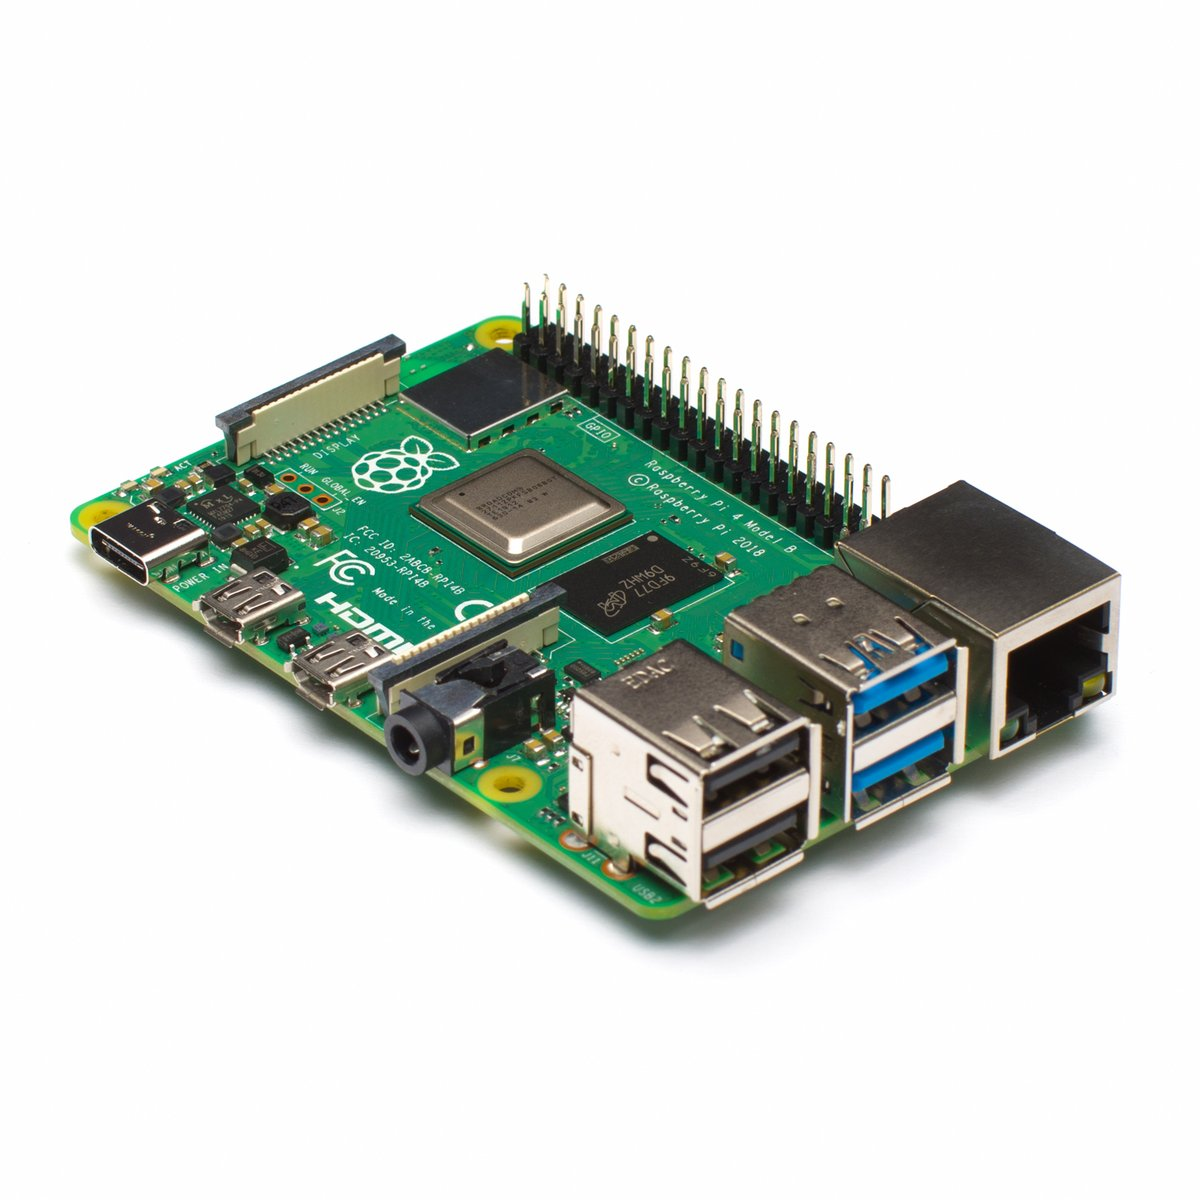
\includegraphics[width=0.85\textwidth]{Images/4-Methods/RPi4.jpg}
			\end{center}
			\caption{Raspberry Pi 4 Model B}
			\label{fig:rpi4Im}
		\end{subfigure}
		\begin{subfigure}[b]{.45\textwidth}
			\begin{center}
				\begin{tikzpicture}[font=\small,thick]
					\node[draw, text centered, fill=white!30,
					align=center,
					minimum width=3cm,
					minimum height=1cm,
					] (block0) { Raspberry Pi 4};
					
					\node[draw,text centered,fill=white!30,rounded corners,
					below=0.5cm of block0, align=center,
					minimum width=2.5cm,
					minimum height=1cm,
					] (block1) { \gls{HRP} Automower };
					
					\node[above=of block0] (block) { };
					
					\node[draw,text centered,fill=yellow!30,rounded corners,
					left=0.1cm of block,
					align=center,
					minimum width=2.5cm,
					minimum height=1cm,
					] (block2) { Phidget \glspl{IMU}};
					
					\node[draw,text centered,fill=green!30,rounded corners,
					right=0.1cm of block,
					align=center,
					minimum width=2.5cm,
					minimum height=1cm,
					] (block3) { Camera};
					
					\node[below=of block1] (blockk) { };
					
					\node[draw,text centered,fill=white!30,rounded corners,
					left=0.1cm of blockk,
					align=center,
					minimum width=2.5cm,
					minimum height=1cm,
					] (block4) { Wheel Encoder};
					
					\node[draw,text centered,fill=white!30,rounded corners,
					right=0.1cm of blockk,
					align=center,
					minimum width=2.5cm,
					minimum height=1cm,
					] (block5) { Automower \gls{GNSS}};
					
					% Arrows
					\draw[latex-] (block0) edge (block1);
					\draw[latex-] (block0) edge (block2);
					\draw[latex-] (block0) edge (block3);
					\draw[latex-] (block1) edge (block4);
					\draw[latex-] (block1) edge (block5);
				\end{tikzpicture}
				\caption[Caption]{Raspberry Pi 4 configuration \centering}
			\end{center}
			\label{fig:RPi4Conf}
		\end{subfigure}
		\caption{Raspberry Pi 4}
		\label{fig:RPi4}
	\end{center}
\end{figure}


\subsection{Raspberry Pi 3}
\noindent
On this device, running Ubuntu 20, the Phidgets GPS sensors will be attached.


\begin{figure}[!ht]
	\begin{subfigure}[b]{.5\textwidth}
		\begin{center}
			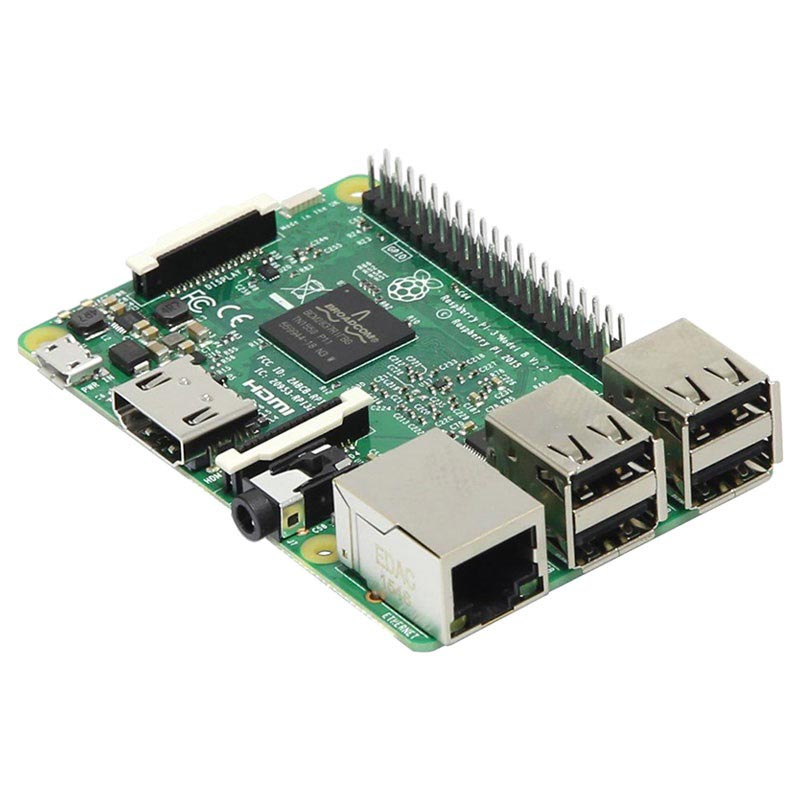
\includegraphics[width=0.5\textwidth]{Images/4-Methods/RPi3.jpg}
		\end{center}
		\caption{Raspberry Pi 3 Model B}
		\label{fig:rpi3Im}
	\end{subfigure}%
	\begin{subfigure}[b]{.45\textwidth}
		\begin{center}
			\begin{tikzpicture}[font=\small,thick]
				\node[draw, text centered, fill=white!30,
				align=center,
				minimum width=3cm,
				minimum height=1cm,
				] (block0) { Raspberry Pi 3};
				
				\node[draw,text centered,fill=cyan!30,rounded corners,
				above=0.5cm of block0, align=center,
				minimum width=2.5cm,
				minimum height=1cm,
				] (block1) { Phidget \glspl{GPS} };
				% Arrows
				\draw[latex-] (block0) edge (block1);
			\end{tikzpicture}
			\caption[Caption]{Raspberry Pi 3 configuration \centering}
		\end{center}
		\label{fig:RPi3Conf}
	\end{subfigure}
	\caption{Raspberry Pi 3}
	\label{fig:RPi3}
\end{figure}


\section{Adaptive Sensor Models}
\noindent Check for new measurements in background and dynamically create the components for the update step

\subsection{Wheel Encoder Model}

\noindent
It is included in the motor of the wheel of the \gls{ALM}, inside the Motor Kit shown in \ref{fig:wheelenc}.
Measure the wheel displacement and provide \gls{WO}, as explained in \ref{ch:methods}.


The performances have been examined and are available below.

\begin{figure}[!ht]
	\begin{center}
		\begin{subfigure}[b]{.5\textwidth}
			\centering
			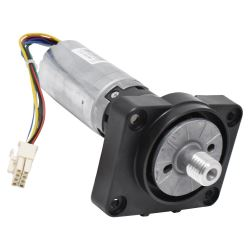
\includegraphics[width=0.75\textwidth]{Images/4-Methods/MotorEnc.jpeg}
			\caption{Motor Kit Automower 450X }
			\label{fig:wheelenc}
		\end{subfigure}%
		\begin{subfigure}[b]{.45\textwidth}
			\begin{center}
				\label{tab:evalWheels}
				\begin{tabular}{|c||S|}
					\hline
					\centering{\textbf{Aspect}} &  \multicolumn{1}{c|}{\textbf{Value}} \\
					\hline
					\hline
					\centering{Frequency} &  \SI{200}{Hz} \\
					\hline
					\centering{$\boldsymbol \eta_v$} &  \SI{0.02}{\meter/\second} \\
					\hline
					\centering{$\boldsymbol \eta_{\omega}$} & \SI{0.02}{\radian/\second} \\
					\hline
				\end{tabular}
				\caption{Sensor's performance}
			\end{center}
		\end{subfigure}
		\caption{Wheel Encoder }
		\label{fig:wheel}
	\end{center}
\end{figure}

They are mounted in the wheel axis on both wheels.

\noindent
Through the usage of wheel encoders attached to both these wheels, an estimated velocity for them is calculated and used to determine its pose.
This open-loop technique to determine the position and orientation is called \gls{DR}, as the new pose is estimated by using the last known pose and the new speed measurements.

The wheel encoders attached on each wheel provide an estimate of the number of pulses they detected. These encoder pulses need to be translated to an approximated wheel displacement through the transformation constant $C_{D}$ provided by equation \ref{eq:wheel_meter}.
\begin{equation}
C_{D} = \frac{\pi \cdot W_D }{E_T}
\label{eq:wheel_meter}
\end{equation} where $W_D$ is the estimated length of the wheel diameter and $E_T$ is the encoder time resolution.
This value is used to derive the velocity of each wheel separately, $\dot \delta_L$ and $\dot \delta_R$, by multiplying their encoder pulses, $E_L$ and  $E_R$ respectively, with transformation constant and dividing it using the time delay $\Delta_t$, as in equation \ref{eq:wheel_disp}.
\begin{equation}
\dot \delta_{L} = \frac{C_D \cdot E_L}{\Delta_t}  \qquad
\dot \delta_{R} = \frac{C_D \cdot E_R}{\Delta_t}
\label{eq:wheel_disp}
\end{equation}

Using these single wheel displacements, it is possible to calculate the linear velocity along the $x$ axis, $v$, and the angular velocity on the $z$ axis, $\omega$, with respect to the mobile robot frame using equations \ref{eq:disp}:
\begin{equation}
    v =\frac{\dot \delta_{R} + \dot \delta_{L} }{2} \qquad \omega = \frac{\dot \delta _{R} - \dot \delta_{L}}{B_W}
\label{eq:disp}
\end{equation} where $B_W$ is the estimated length of the base width of the back wheel axis.


These forward kinematics equations of this differential drive mobile robot are used to update the pose of the mobile robot, from time $t$ after a time step $\Delta_t$ to time $t+1$, in the global coordinate frame with the Euler first-order differential approximation~\cite{braun_first-order_1993}, as shown in equation \ref{eq:eulerWheel}.

\begin{equation}
\begin{bmatrix} x_{t + 1} \\ y_{t + 1} \\ \theta _{t + 1} ~ \end{bmatrix}
=
\begin{bmatrix} {x_t} \\ {y_t} \\ {\theta _t}  \end{bmatrix}
+
\begin{bmatrix}  \cos (\theta _t ) & 0\\  \sin (\theta _t ) & 0 \\ 0 & 1 \end{bmatrix}
\cdot
\begin{bmatrix} v \\ \omega \end{bmatrix} \cdot
\Delta_t
\label{eq:eulerWheel}
\end{equation}


This method however is subject to multiple errors and inaccuracies, as the measurements and time delays will never be perfect.
The systematic errors can be given by imperfectness of robot model as impreciseness in the wheel diameters or wheel base measures, which are used to estimate the movements.
However, the presence of non-systematic random errors as result of usage of imperfect measurements are more difficult to model, e.g. wheel slippage, uneven terrain, and external forces applied.
The accumulative characteristic of these errors will break the stability of the system, making the estimate to drift after a period of time.
These conditions render this \gls{DR} model not adequate to determine the pose of the mobile robot, but its estimate could be used anyway to improve the positioning system.


\begin{align}
\mathbf{v}_{Enc_t} & = \mathbf{v} &
\boldsymbol \omega_{Enc_t} & = \boldsymbol \omega
\end{align}


Measurements vector with uncertainty vector
\begin{align}
\mathbf{Z}
=
\begin{bmatrix}
\mathbf{v}_{Enc_t} \\
\boldsymbol \omega_{Enc_t}
\end{bmatrix}^T
& \quad
\mathbf{R}
=
\begin{bmatrix}
\eta_{\mathbf{v}_{Enc}} \\
\eta_{\boldsymbol \omega}
\end{bmatrix}^T
\end{align}
where $ \omega_{\mathbf{x}_{Enc}} = \omega_{\mathbf{y}_{Enc}} = 1$ and
$ \omega_{\boldsymbol \theta_{Enc}} = \pi/180 $ , experimentally derived.


Measurement Matrix
\begin{equation}
H
=
\begin{bmatrix}
0 & 0 & 0 & 1 & 0 & 0 \\
0 & 0 & 0 & 0 & 1 & 0
\end{bmatrix}
\end{equation}

Measurement Jacobian Matrix
\begin{equation}
J_H
=
\begin{bmatrix}
0 & 0 & 0 & 1 & 0 & 0 \\
0 & 0 & 0 & 0 & 1 & 0
\end{bmatrix}
\end{equation}


\subsection{GNSS receiver Model}


\noindent Measure the satellite positions to estimate its absolute position global values in the global coordinate frame.

Different \glspl{GNSS} are available.
A \gls{GPS} receiver is embedded in the \gls{HRP}, shown in \ref{fig:autogps}.
Moreover, two additional \gls{GPS} receivers has been added, shown in \ref{fig:phigps}.

\begin{figure}[!ht]
	\begin{center}
		\begin{subfigure}[b]{.5\textwidth}
			\centering
			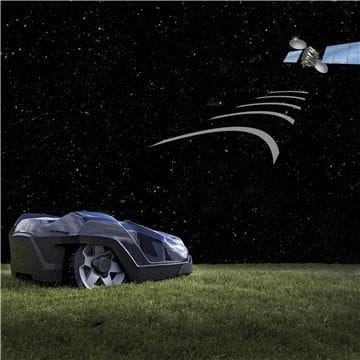
\includegraphics[width=0.75\textwidth]{Images/4-Methods/AutomowerGPS.jpeg}
			\caption{Automower 450X GPS}
			\label{fig:autogps}
		\end{subfigure}%
		\begin{subfigure}[b]{.45\textwidth}
			\begin{center}
				\label{tab:evalAutoGPS}
				\begin{tabular}{|c||S|}
					\hline
					\centering{\textbf{Aspect}} &  \multicolumn{1}{c|}{\textbf{Value}} \\
					\hline
					\hline
					\centering{Frequency} &  \SI{1}{Hz} \\
					\hline
					\centering{$\boldsymbol \eta_x$} &  \SI{0.02}{\meter/\second} \\
					\hline
					\centering{$\boldsymbol  \eta_y$} &  \SI{0.02}{\meter/\second} \\
					\hline
					\centering{$\boldsymbol \eta_{\theta}$} & \SI{0.02}{\radian/\second} \\
					\hline
				\end{tabular}
				\caption{Sensor's performance}
			\end{center}
		\end{subfigure}
		\caption{\glspl{GNSS} receivers adopted}
		\label{fig:gpssensorauto}
	\end{center}
\end{figure}

The performances of PhidgetGPS ID: 1040\_0B have been examined and are available below.

\begin{figure}[!ht]
	\begin{center}
		\begin{subfigure}[b]{.5\textwidth}
			\centering
			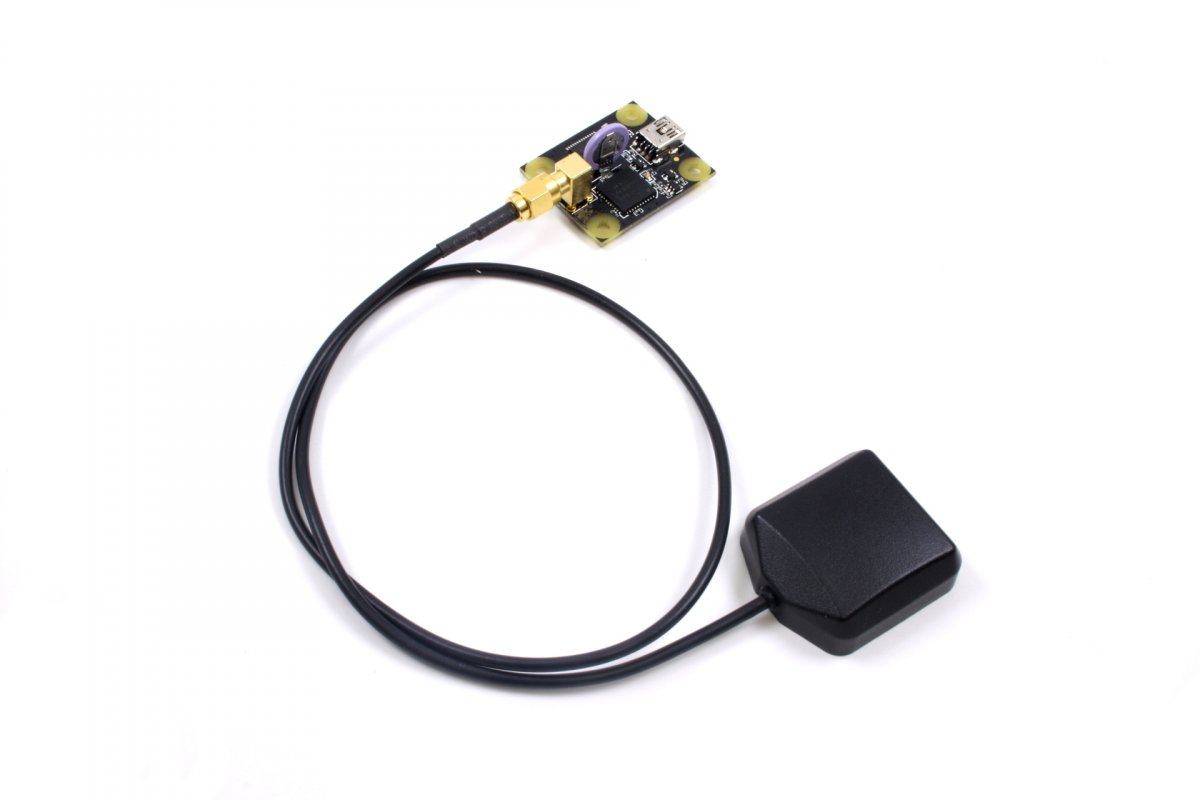
\includegraphics[width=1\textwidth]{Images/4-Methods/1040_0B_Alt2.jpg}
			\caption{Performances}
			\label{fig:phigps}
		\end{subfigure}
		\begin{subfigure}[b]{.45\textwidth}
			\begin{center}
				\label{tab:evalPhiGPS}
				\begin{tabular}{|c||S|}
					\hline
					\centering{\textbf{Aspect}} &  \multicolumn{1}{c|}{\textbf{Value}} \\
					\hline
					\hline
					\centering{Frequency} &  \SI{5}{Hz} \\
					\hline
					\centering{$\boldsymbol \eta_x$} &  \SI{0.02}{\meter/\second} \\
					\hline
					\centering{$\boldsymbol  \eta_y$} &  \SI{0.02}{\meter/\second} \\
					\hline
					\centering{$\boldsymbol \eta_{\theta}$} & \SI{0.02}{\radian/\second} \\
					\hline
				\end{tabular}
				\caption{Sensor's performance}
			\end{center}
		\end{subfigure}%
		\caption{\glspl{GNSS} receivers}
		\label{fig:gpssensorphi}
	\end{center}
\end{figure}



It is mounted in front, at coordinate x,y,z with orientation theta with respect to the robot coordinate frame.

\noindent The measures obtained by the \gls{GNSS} receiver are transformed from WSG-84 degrees to local coordinates as specified below.

Using specific math equations derived by~\cite{Vincenty}, first a transformation from the geodetic coordinates in WSG-84 degrees estimated by the GPS receiver sensors to the ECEF coordinates is implemented.
It is done so both for the initial coordinate and then used to check the difference with the ECEF translation from the geodetic coordinates of the successive reading of the GPS receiver.


%GPS positioning is in the global coordinate system WGS84 [18].

From World Geodetic System: WGS 84 values
\begin{align}
    R_E &= 6378137 && \text{Equatorial radius (\SI{}{\meter})} \\
    R_P &= 6356752.3142 && \text{Polar radius (\SI{}{\meter})}
\end{align}

From which the following can be derived the following values necessary for the next algorithms:
\begin{align}
    F_R &= \frac{R_E - R_P}{R_E} &
    E_R &= F_R \cdot (2-F_R)
\end{align}

Using these values it is possible to transform from Geodetic WSG-84 Coordinates to ECEF coordinates using the  Algorithm specified in \ref{alg:ecef}.


\begin{algorithm}[ht!]
\caption{Geodetic to ECEF Coordinates }
\label{alg:ecef}
  \hspace*{\algorithmicindent} \textbf{Input:} Latitude and Longitude ($lat$, $lon$) in WSG-84 degrees\\
  \hspace*{4em} Altitude ($h$) in meters\\
  \hspace*{\algorithmicindent} \textbf{Output:} ECEF Coordinates in meters ($x$, $y$, $z$)
  %\KwData{Testing set $x$}
  %$\sum_{i=1}^{\infty} := 0$ \tcp*{this is a comment}
  %\tcc{Transform latitude and longitude}
  \begin{algorithmic}[1]
  \STATE $N = \cfrac{EqR}{\sqrt{1 - E_R \cdot \sin(lat)^2}}$
  \STATE $x = (h + N) \cdot \sin(lat) \cdot \cos(lon)$
  \STATE $y = (h + N) \cdot \cos(lat) \cdot \sin(lon)$
  \STATE $z = (h + (1 - e\_sq) \cdot N) \cdot \sin(lat)$
  \STATE return $x$, $y$, $z$
    \end{algorithmic}
\end{algorithm}

Finally, by exploiting the previous algorithm, it is possible to transform the Current Geodetic Coordinates into Local Coordinates by using some Reference Geodetic Coordinates and Algorithm \ref{alg:local}.
\begin{algorithm}[ht!]
\caption{Geodetic to Local using Current and Reference Coordinates}
\label{alg:local}
    \hspace*{\algorithmicindent} \textbf{Input:} Current Latitude and Longitude ($latC$, $lonC$)\\
        \hspace*{5em} in WSG-84 degrees\\
    \hspace*{4em} Current Altitude ($hC$) in meters\\
    \hspace*{4em} Reference Latitude and Longitude ($latR$, $lonR$)\\
        \hspace*{5em} in WSG-84 degrees\\
    \hspace*{4em} Reference Altitude ($hR$) in meters \\
    \hspace*{\algorithmicindent} \textbf{Output:} Local Coordinates in meters ($\Delta x$, $\Delta y$, $\Delta z$)
  \begin{algorithmic}[1]
    \STATE $xC$, $yC$, $zC$ = Geodetic to ECEF Coordinates ($latC$, $lonC$, $hC$)
    \STATE $xR$, $yR$, $zR$ = Geodetic to ECEF Coordinates ($latR$, $lonR$, $hR$)
    \STATE $xD = xC - xR$
    \STATE $yD = yC - yR$
    \STATE $zD = zC - zR$
    \STATE $\Delta x = -~\sin(lonR)~\cdot~xD~+~\cos(latR)~\cdot~yD$
    \STATE $\Delta y = -~\cos(lonR)~\cdot~\sin(latR)~\cdot~xD~-~\sin(latR)~\cdot~\sin(lonR)~\cdot~yD~+ \hspace*{3em} \cos(latR)~\cdot~zD$
    \STATE $\Delta z = \cos(latR)~\cdot~\cos(lonR)~\cdot~xD~+~\cos(latR)~\cdot~\sin(lonR)~\cdot~yD~+  \hspace*{3em} \sin(latR)~\cdot~zD$
    \STATE return $\Delta x$, $\Delta y$, $\Delta z$
    \end{algorithmic}

\end{algorithm}

In order to get the mean using the first measurements before the first command to move the automower, those values are stored in $\mu_{lat}$ and $\mu_{long}$.

The formula used to obtain the distance between this mean value and the current value of the gps measurements is defined below.
\begin{align}
\mathbf{x}_{GPS_t} & = \text{geodetic2enu}( latC - latR)\\
\mathbf{y}_{GPS_t} & = \text{geodetic2enu}( longC - lonR)
\end{align}

Then the orientation $z_{\boldsymbol \theta_{GPS_t}}$ is obtained by computing the direction between consecutive measurements.
\begin{equation}
z_{\boldsymbol \theta_{GPS_t}} = \arctan(\mathbf{y}_{GPS_{t-1}} - \mathbf{y}_{GPS_t}, \mathbf{x}_{GPS_{t-1}} - \mathbf{x}_{GPS_t} )
\end{equation}

"""In this section we shall assume that wrapping operation
amounts to enforcing the angular variable to be in the [$-\pi$, $\pi$]
interval, and we designate this operation as follows
\begin{equation}
w_{\pi}(x) = mod(x + \pi, 2\pi) - \pi
\end{equation}

Note that when computing the difference between two angular
variables, the wrapping effect of the circle should be taken into
account, e.g., the difference between 178° and -178° should
evaluate to 4°. This is achieved by the function $w_{\pi}(x)$ when the difference
is given as the argument, i.e., difference between two angles
x and y is computed as $w_{\pi}(x-y)$, as defined in~\cite{markovic_wrapping_2017}.
"""
\begin{equation}
	\boldsymbol \theta_{GPS_t} = \boldsymbol \theta_{t} + w_{\pi}(z_{\boldsymbol \theta_{GPS_t}} - \boldsymbol \theta_{t})
\end{equation}

Measurements vector with uncertainty vector
\begin{align}
\mathbf{Z}
=
\begin{bmatrix}
\mathbf{x}_{GPS_t} \\
\mathbf{y}_{GPS_t} \\
\boldsymbol \theta_{GPS_t} \\
\end{bmatrix}^T
& \quad
\mathbf{R}
=
\begin{bmatrix}
\omega_{\mathbf{x}_{GPS}} \\
\omega_{\mathbf{y}_{GPS}} \\
\omega_{\boldsymbol \theta_{GPS}} \\
\end{bmatrix}^T
\end{align}
where $ \omega_{\mathbf{x}_{GPS}} = \omega_{\mathbf{y}_{GPS}} = \text{HDOP} = \sqrt{\sigma_x^2 + \sigma_y^2}$ and
$ \omega_{\boldsymbol \theta_{GPS}} = \pi/8 $ , experimentally derived.

Measurement Matrix
\begin{equation}
H
=
\begin{bmatrix}
1 & 0 & 0 & 0 & 0 & 0 \\
0 & 1 & 0 & 0 & 0 & 0 \\
0 & 0 & 1 & 0 & 0 & 0 \\
\end{bmatrix}
\end{equation}

Measurement Jacobian Matrix
\begin{equation}
J_H
=
\begin{bmatrix}
1 & 0 & 0 & 0 & 0 & 0 \\
0 & 1 & 0 & 0 & 0 & 0 \\
0 & 0 & 1 & 0 & 0 & 0 \\
\end{bmatrix}
\end{equation}



\subsection{IMU Model}


\noindent Measure the angular velocity, acceleration, and magnetic fields in the three orthogonal axis.

This PhidgetSpatial Precision 3/3/3 High Resolution - ID: 1044\_1B, shown in \ref{fig:spatial}, has a 3-axis accelerometer, gyroscope and compass with high resolution readings at low magnitudes.

The performances have been examined and are available below.

\begin{figure}[!ht]
	\begin{center}
		\begin{subfigure}[b]{.5\textwidth}
			\begin{center}
				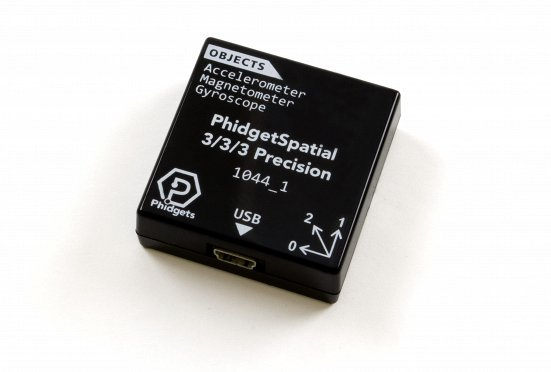
\includegraphics[width=1\textwidth]{Images/4-Methods/1044_1B.jpg}
			\end{center}
			\caption{Performances}
			\label{fig:spatial}
		\end{subfigure}
		\begin{subfigure}[b]{.45\textwidth}
			\begin{center}
				\label{tab:evalPhiIMU}
				\begin{tabular}{|c||S|}
					\hline
					\centering{\textbf{Aspect}} &  \multicolumn{1}{c|}{\textbf{Value}} \\
					\hline
					\hline
					\centering{Frequency} &  \SI{250}{Hz} \\
					\hline
					\centering{$\boldsymbol \eta_{\omega}$} & \SI{0.02}{\radian/\second} \\
					\hline
					\centering{$\boldsymbol \eta_{a}$} & \SI{0.02}{\meter/\second \squared} \\
					\hline
				\end{tabular}
				\caption{Sensor's performance}
			\end{center}
		\end{subfigure}%
		\caption{\glspl{IMU}}
		\label{fig:imusensorphi}
	\end{center}
\end{figure}

It is mounted in front, at coordinate x,y,z with orientation theta with respect to the robot coordinate frame.

"""As a general rule the closer is the IMU to the Centre of Gravity/Rotation the better; is to bear in mind that compensation for position offset reduces overall accuracy."""

The mobile robot is constrained to move and rotate around its center of rotation, in a way that the displacement of the imu will not lower the performance, moreover, the angular velocity is the same for the whole robot, so the measured angular velocity can be fused directly.


Measurements vector, as obtained by IMU, with uncertainty vector.

The measurements obtained by the IMU are related to its own frame, so these measures need to be translated into the correct robot frame, by using the Rotation matrix.
\begin{align}
	\omega_r &= R_i^r \cdot \omega_i & \mathbf{a}_r &= R_i^r \cdot \mathbf{a}_i
\end{align}

Using the newly obtained calibrated measurements, the measurement matrix and related noise matrix are defined as follows.
\begin{align}
\mathbf{Z}
&=
\begin{bmatrix}
\boldsymbol \omega_{IMU_t} \\
\mathbf{a}_{IMU_t} \\
\end{bmatrix}^T
& 
\mathbf{R}
&=
\begin{bmatrix}
\eta_{\boldsymbol \omega_{IMU}} \\
\eta_{\mathbf{a}_{IMU}} \\
\end{bmatrix}^T
\end{align}
where $ \omega_{\dot{\boldsymbol \theta}_{IMU}} = 1$ and
$ \omega_{\mathbf{a}_{IMU}} = 4 $ , experimentally derived.


Measurement Matrix
\begin{equation}
H
=
\begin{bmatrix}
0 & 0 & 0 & 0 & 1 & 0 \\
0 & 0 & 0 & 0 & 0 & 1 \\
\end{bmatrix}
\end{equation}

Measurement Jacobian Matrix
\begin{equation}
J_H
=
\begin{bmatrix}
0 & 0 & 0 & 0 & 1 & 0 \\
0 & 0 & 0 & 0 & 0 & 1 \\
\end{bmatrix}
\end{equation}

\subsection{Camera Model}


\noindent Measure the displacement of the camera \gls{F2F} and provide \gls{VO}.
The device that is used is the Intel® RealSense™ depth camera D435, shown in Figure \ref{fig:d435}.
It provides \gls{RGBD} images, i.e. both \gls{RGB} and depth information.

"The Intel® RealSense™ depth camera D435 is a stereo solution, offering quality depth for a variety of applications. It's wide field of view is perfect for applications such as robotics or augmented and virtual reality, where seeing as much of the scene as possible is vitally important."

\begin{figure}[!ht]
	\begin{center}
		\begin{subfigure}[b]{.5\textwidth}
			\begin{center}
				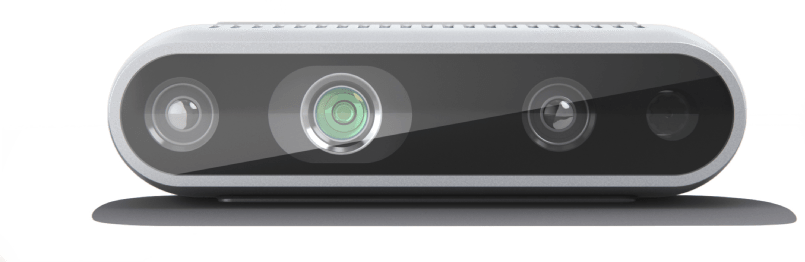
\includegraphics[width=0.85\textwidth]{Images/4-Methods/d435i-1.png}
			\end{center}
			\caption{\gls{RGBD} Camera Performances}
			\label{fig:d435}
		\end{subfigure}
		\begin{subfigure}[b]{.45\textwidth}
			\begin{center}
				\label{tab:evalCamera}
				\begin{tabular}{|c||S|}
					\hline
					\centering{\textbf{Aspect}} &  \multicolumn{1}{c|}{\textbf{Value}} \\
					\hline
					\hline
					\centering{Frequency} &  \SI{5}{Hz} \\
					\hline
					\centering{$\boldsymbol \eta_{v}$} & \SI{0.02}{\meter/\second} \\
					\hline
					\centering{$\boldsymbol \eta_{\omega}$} & \SI{0.02}{\radian/\second} \\
					\hline
				\end{tabular}
				\caption{Sensor's performance}
			\end{center}
		\end{subfigure}%
		\caption{Camera}
		\label{fig:camera_sensor}
	\end{center}
\end{figure}

It is mounted in front, at coordinate x,y,z with orientation theta with respect to the robot coordinate frame.

Using the \gls{RTABMAP} package\footnote{\url{http://introlab.github.io/rtabmap/}}\cite{6094602} \cite{labbe_rtab-map_2019}, more specifically the \gls{ROS} version 0.20.9 for \gls{ROS} Noetic.


\noindent 
Measurements vector, as obtained by the \gls{RTABMAP} package in \gls{ROS}.
Moreover, it also provides its own uncertainty vector error based on the uncertainty of the estimation over the images.

Odometry velocities merged, as the drift may still be an issue.


Measurements vector with uncertainty vector
\begin{align}
\mathbf{Z}
=
\begin{bmatrix}
\mathbf{v}_{Vis_t} \\
\boldsymbol \omega_{Vis_t}
\end{bmatrix}^T
& \quad
\mathbf{R}
=
\begin{bmatrix}
\eta_{\mathbf{v}_{Vis}} \\
\eta_{\boldsymbol \omega_{Vis}}
\end{bmatrix}^T
\end{align}
where $ \omega_{\mathbf{x}_{Vis}} = \omega_{\mathbf{y}_{Vis}} = 1$ and
$ \omega_{\boldsymbol \theta_{Vis}} = \pi/180 $ , experimentally derived.


Measurement Matrix
\begin{equation}
H
=
\begin{bmatrix}
0 & 0 & 0 & 1 & 0 & 0 \\
0 & 0 & 0 & 0 & 1 & 0
\end{bmatrix}
\end{equation}

Measurement Jacobian Matrix
\begin{equation}
J_H
=
\begin{bmatrix}
0 & 0 & 0 & 1 & 0 & 0 \\
0 & 0 & 0 & 0 & 1 & 0
\end{bmatrix}
\end{equation}


%\section{Localisation Configuration}
\section{Sensor Fusion Model}
\label{sec:locConf}
\noindent
The localisation module is based on the merging of the information derived by the kinematic model, the control commands, and the sensors' measurements.
The sensor fusion algorithm \gls{AEKF} has been chosen for its time performances and reliability.
It improves the \gls{KF} allowing for the management of non-linear systems and the possibility to account for dynamic sensors' noise.
It is defined as a Discrete time system, running with a frequency defined by the value $Hz$.
Its implementation is hereby defined, starting from the Prediction phase, the different Measurements models of the heterogeneous sensors, and the Correction phase.


The system will start with all the state variables set to $0$ and a know initial Covariance matrix $P_0$ set as an Identity $I$ multiplied by $1^{-3}$, i.e. diagonal matrix with those values.

\subsection{Prediction Model}

\noindent The prediction phase is driven by the kinematic model, as it is defined in Figure \ref{fig:TikzKine}, following the conclusions of~\cite{801027}.

As assumption, the system will follow a Constant Velocity Model.

The state variables needed to provide the most accurate positioning in a \gls{2D} environment are defined in \eqref{eq:state-transf}.
\begin{equation}
	\label{eq:state-transf}
	\mathbf{X}_t=
	\begin{bmatrix}
		\mathbf{x}_t & \mathbf{y}_t & \boldsymbol \theta_t & \mathbf{v}_t & \boldsymbol \omega_t
	\end{bmatrix} ^T
\end{equation}
From the definition of the Kinematic Model in Figure \ref{fig:TikzKine}, the first three positional elements, i.e. $\mathbf{x}_t$, $\mathbf{y}_t$, and $\boldsymbol \theta_t$, are related to the global frame. Instead the following inertial elements, i.e. $\mathbf{v}_t$, $\boldsymbol \omega_t$, and $\mathbf{a}_t$ are defined from the robot frame.
As assumption, the system will start with a known initial state $\mathbf{X}_0$ of mean $0$ for each element.

%\subsubsection{Transition}
The transition matrix related to the states defined in Equation \eqref{eq:state-transf} and to the kinematic model of Figure \ref{fig:TikzKine} is given by \eqref{eq:trans-mat}.
\begin{equation}
	\label{eq:trans-mat}
	A_t
	=
	\begin{bmatrix}
		1 & 0 & 0 & \cos(\boldsymbol \theta_t) \cdot \Delta_t & 0 \\
		0 & 1 & 0 & \sin(\boldsymbol \theta_t) \cdot \Delta_t & 0 \\
		0 & 0 & 1 & 0 & \Delta_t  \\
		0 & 0 & 0 & 1 & 0 \\
		0 & 0 & 0 & 0 & 1 & 
	\end{bmatrix}
\end{equation}
where $\boldsymbol \Delta_t$ is the time step used by the \gls{AEKF}.
It accounts for the transformation of the linear velocity, angular velocity, and the linear acceleration to update the position states that are used as \gls{DOF}, as defined in Equation \eqref{eq:dof}.

%\subsubsection{Control}
As defined in Section \ref{ssec:kin_a}, the \gls{ALM} is controlled using the linear and angular velocities.
This configuration is used by the \gls{AEKF} to improve the Prediction step using the following Control matrix $B$ and states $\mathbf{u}_t$, as defined in Equations \eqref{eq:cmd}.
\begin{align}
	\label{eq:cmd}
	B &=
	\begin{bmatrix}
		0 & 0 \\
		0 & 0\\
		0 & 0\\
		\Delta_t & 0\\
		0 & \Delta_t
	\end{bmatrix}
	&
	\mathbf{u}_t &=
	\begin{bmatrix}
		\textbf{cmd}_{\mathbf{v}} - \mathbf{v}_t  \\
		\textbf{cmd}_{\boldsymbol \omega} - \boldsymbol \omega_t \\[0.3em]
	\end{bmatrix}
\end{align}
where $\Delta_t$ is the time step of the \gls{AEKF} used to make the transition from command received and actual actuation more smooth by dynamically scaling the innovation, and $\textbf{cmd}_{\mathbf{v}}$ and  $\textbf{cmd}_{\boldsymbol \omega}$ are the commands sent to the robot. % obtained by a specific topic. 
\com{
	and $\mathbf{s}_{i}$ is used to make the transition from command received and actual actuation more smooth by limiting the innovation given by the respective control through a scaling value equal to the frequency of the system: $\mathbf{s}_i = \frac{1}{Hz}$, with $Hz$ as the frequency of the \gls{AEKF}.
}

%\subsubsection{Uncertainty}
\com{
	The noise vector related to the state variables estimate is adaptively defined by $\boldsymbol \eta$ as in \eqref{eq:noise-p}.
	\begin{equation}
		\label{eq:noise-p}
		\boldsymbol \eta
		=
		\begin{bmatrix}
			\boldsymbol \eta_{\mathbf{x}}  &
			\boldsymbol \eta_{\mathbf{y}} &
			\boldsymbol \eta_{\boldsymbol \theta}  &
			\boldsymbol \eta_{\mathbf{v}} &
			\boldsymbol \eta_{\boldsymbol \omega} &
			\boldsymbol \eta_{\mathbf{a}}
		\end{bmatrix} ^T
	\end{equation}
	where $\eta_i \sim \mathcal{N}(\mu_i,\,\sigma_{ii}^{2})$ with $\mu_i = 0$, $\sigma_{ii}^2 = 0.1$, and $ i = \{ \mathbf{x} , \mathbf{y} , \boldsymbol \theta , \mathbf{v} , \boldsymbol \omega , \mathbf{a} \}$
	where $\sigma_{\mathbf{xx}}^2 = \sigma_{\mathbf{yy}}^2 = \sigma_{\mathbf{\boldsymbol \theta \boldsymbol \theta}}^2  = \cfrac{{\boldsymbol \Delta_t}^2}{2}$, and $\boldsymbol \Delta_t$ is the time step used by the \gls{AEKF}.
}

The prediction of the estimate regarding the state variables is defined in the \gls{KF} by equation \eqref{eq:pred-state-formula}.
	\begin{equation}
		\label{eq:pred-state-formula}
		\mathbf{X}_{p} = A \cdot \mathbf{X}_t + B \cdot \mathbf{u}_t + \boldsymbol \eta
	\end{equation}

%\subsubsection{Linearisation}

As the Kalman Filter is not able to deal with non-linear systems, the Jacobian of the Transition matrix must be obtained to linearise the non-linear equations with a first-order Taylor expansion.
The resulting matrix $J_A$, defined in \eqref{eq:j-a}, can then be used by the \gls{AEKF} for the prediction of the Covariance matrix.
\begin{equation}
	\label{eq:j-a}
	J_A
	=
	\begin{bmatrix}
		1 & 0 & 0 & -\sin(\boldsymbol \theta_t) \cdot \Delta_t & 0  \\
		0 & 1 & 0 & ~\cos(\boldsymbol \theta_t) \cdot \Delta_t & 0  \\
		0 & 0 & 1 & 0 & \Delta_t \\
		0 & 0 & 0 & 1 & 0  \\
		0 & 0 & 0 & 0 & 1  
	\end{bmatrix}
\end{equation}

The prediction noise matrix, given by $Q$ in Equation \eqref{eq:q-p}, is defined by uncorrelated and zero-mean white noise, with the diagonal elements set dynamically as the related noise of the state variables.
\begin{align}%Continuous White Noise Model
	\label{eq:q-p}
	\tiny
	Q
	=
	\com{
		{\sigma_{\mathbf{xx}}^2} & 0 & 0 & 0 & 0 \\
		0 & \sigma_{\mathbf{yy}}^2 & 0 & 0 & 0 \\
		0 & 0 & \sigma_{\mathbf{\boldsymbol \theta \boldsymbol \theta}}^2 & 0 & 0 \\
		0 & 0 & 0 & \sigma_{\mathbf{vv}}^2 & 0 \\
		0 & 0 & 0 & 0 & \sigma_{{\boldsymbol \omega}{\boldsymbol \omega}}^2
	}
	\begin{bmatrix}
		{\sin(\boldsymbol \theta_t)}^2 \cdot \cfrac{{\Delta_t}^2}{2} & - \sin(\boldsymbol \theta_t) \cdot \cos(\boldsymbol \theta_t) \cdot \cfrac{{\Delta_t}^2}{2} & 0 & - \sin(\boldsymbol \theta_t) \cdot {\Delta_t}^2 & 0 \\
		- \sin(\boldsymbol \theta_t) \cdot \cos(\boldsymbol \theta_t) \cdot {\Delta_t}^2 & \cos(\boldsymbol \theta_t)^2 \cdot \cfrac{{\Delta_t}^2}{2} & 0 & \cos(\boldsymbol \theta_t) \cdot {\Delta_t}^2 & 0 \\
		0 & 0 & \cfrac{{\Delta_t}^2}{2} & 0 & { \Delta_t}^2 \\
		- \sin(\boldsymbol \theta_t) \cdot {\Delta_t}^2 & \cos(\boldsymbol \theta_t) \cdot {\Delta_t}^2 & 0 & { \Delta_t} & 0 \\
		0 & 0 & { \Delta_t}^2 & 0 & { \Delta_t}
	\end{bmatrix}
	\cdot
	\sigma_a
\end{align}
where $\boldsymbol \Delta_t$ is the time step used by the \gls{AEKF} and $\sigma_a$ is the mean of the acceleration along the $X$ axis of the robot frame, as measured by the \glspl{IMU} or given by the costant $g = 9.81$ if no \glspl{IMU} are available, as done in ~\cite{king_low_2008}.
This formulation is provided to model the error in the process as a function of the acceleration.
The diagonal assumption means that the errors between variables are not directly associated, but their relationships and related propagation of errors will appear through the transition matrix Jacobian  $J_A$~\cite{king_low_2008}.

Finally, the predicted covariance matrix, defined by $\hat{P}_{t+1}$ is updated during the prediction using the Jacobian $J_A$ and the process noise covariance $Q$, as in Equation \eqref{eq:cov-p}.
\begin{align}
	\label{eq:cov-p}
	%P_0 &= I \cdot 1^{-3} &
	\hat{P}_{t+1} & = J_A \cdot P_t \cdot J_A^T + Q
\end{align}%P_{p} & =  \frac{P_{p} +  P_{p}^T}{2} && \text{To ensure symmetry}


\subsection{Correction Model}

\noindent
Gather all measurements and then use those combined measures for one single correction step, following a batch fusion approach.

Use of thread locks to avoid issues related to out of sequence measurements.

Joseph Form Covariance update is adopted, given the superior numerical performances obtained.
(More time consuming) - Low improvements still relevant to be applied.

\com{
    \lstset{extendedchars=true}
    \begin{lstlisting}[language={Python}, caption={Batch EKF}, label=lst:programmes]
    #  Start node
    #  Subscribe to topics
    #  Update
    #  Get measures
    #  Correct
    #  Sleep to ensure frame rateS
    \end{lstlisting}
}


\section{Mapping Configuration}
\label{sec:mapConf}

\noindent The occupancy grid is defined using \gls{ROS}. It is composed by a grid of cells of dimension \SI{150}{m}~x~\SI{150}{m}, with the center positioned in the middle of this square at position (\SI{75}{m}~,~\SI{75}{m}), and with a resolution of \SI{0.1}{m}. In this way, it will be possible to manage an area of \SI{5000}{m^2} whichever the configuration of the lawn.

\subsection{Virtual Boundary}
\noindent
The external boundaries are defined as $-1$ values, and so if the automower finds itself close to or directly on a cell with a value of $-1$, it will change its orientation and continue on his tasks.
The rest of the cells are initialised with value $50$, meaning that the initial assumption is that the environment is uncertain and that there might be obstacles present within it.

At the first run of the automower, the estimated trajectory derived by the EKF will be used to set the corresponding boundary, i.e. by setting the cells it directly travelled through to $-1$.

After this guided procedure, the automower will have an estimate of its environment configuration and a virtual boundary to delimit its operations.

\subsection{Map Update}
\noindent
After this phase of boundary definition, the \gls{ALM} is left free to roam on that area.
Even if it is defined with cells containing values of $0$, it might still present unexpected objects and those are identified through the collision sensor.

The value of each cell then contains the probability that an object is present in that position, with those values being updated through an average of its previous occupancy probability and the eventuality of collision events detected by the \gls{ALM}.

Each grid cell of the occupancy grid map contains different values of the probabilities that rely on the sonar range information. The probability for occupied grid cell should be equal to (0.98) for the maximum self-belief for various robotics task [3,4,5]. But the probability for the occupied grid cell varied as the range information from sonar varies corresponding to the grid cell under consideration [3].

Mathematical analysis for the investigation of the importance of probabilistic model in occupancy grid mapping is considered that is based on Bayesian technique. Bayesian theorem is an efficient technique to fuse the information of two occupancy grid map on the basis of probabilistic model as shown below.

To do this, conditional independence is assumed between grid cells.


The equation to update the cells is based on the Bayes Theorem.
As defined in \cite{joubert2012adaptive} and \cite{singh_sonar_2019}, then the equation to update it is shown below:
\begin{equation}
    P_{i,j}^{t+1} = \cfrac{P_{i,j}^{t} \cdot P_{env}}{P_{i,j}^{t} \cdot P_{env} + (1-P_{i,j}^{t}) \cdot (1-P_{env})}
\end{equation}
, where $P_{i,j}^{t}$ is the final value of cell $i,j$, $P_{i,j}^{t-1}$ is the previous value of the same cell, and $P_{env}$ is the collision event value.
{\tiny }
This update equation has the important advantage that it is associative and commutative, enabling to incorporate measurements in any order.

\section{Evaluation Framework}
\com{
\todo[inline]{This should also show that you are aware of the social and ethical concerns that might be relevant to your data collection method.)}
}

\label{sec:testing}

\noindent 
The evaluation configuration is defined, showing how the system developed is performing and how its performance are going to be evaluated.

Multiple tests are made.
The teleoperation script available is used to control the mobile robot in velocity.
The measures obtained by an experiments are stored in \gls{ROS} bags which can be used later on to test the filter multiple times with the same experiment.

Different configurations that are going to be tested provide different observabilty performance for the AEKF filter.
observability



Finally, to evaluate if the objectives have been fulfilled and the results can be evaluated as valuable, the following steps are required:
\begin{itemize}
	\item The quantitative measures need to be tested in a real use case experiment, as specified in the research questions.
	\item The data, acquired during these testing phases, will be used and analysed to check if the set of objectives have been reached.
	\item A statistical analysis over multiple experimental tests will provide more reliable results to be presented in the final report.
\end{itemize}


To gather data used to test and analyse the performance of the system, multiple outdoor tests have been carried on.
Some tests have been made to define the calibration of the sensors against a ground truth identified using measure tape.
Some other tests have been made to ensure that the system is behaving accurately while steering.
Some tests have been made to check that the collision events are estimated with an certain degree of precision.

During these tests the rosbag utils provided by ROS has been exploited. Through this service it is possible to store every message sent to the topics, and they can be reused in the future to tune the algorithms.
In this way, the real measurements gathered during outdoor testing can be re evaluated through the play of said messages and using a simulated parameter to reset the clock of ROS framework.



\subsection{Ground Truth Generation}
\label{sec:gt}

\noindent The ground truth is constructed manually by checking the actual path travelled by the robot with the usage of a meter. Setting the experiment and having the robot to follow that path manually, commanding it using the given teleoperation script.


\subsection{Simulation design}
\label{sec:simDesign}

\noindent Simulations will provide an overview of the sensor fusion should behave.

It will use the measures obtained by the Ground Truth.
As a real measure is obtained by a sensors, a simulated measure is generated from the ground truth using a Gaussian white noise to satisfy the Kalman assumptions.

These simulated measures are used by the Kalman filter to offer its estimate.



\subsection{Data Analysis Technique}

\noindent To compare the performances of different configurations, different experiments have been run.
The different performance offered by different configuration is provided comparing the measures of the desired aspects with the frequency of the \gls{EKF}, i.e. at each step of the Sensor Fusion process the estimates of the pose are compared with the Ground Truth.



\subsection{Evaluation Metric}

\noindent \gls{RMSE} is used to compute the performance at each step.
It uses the whole history of errors and then provides its value.
\begin{equation}
    RMSE_j = \sqrt{ \frac{1}{N}\sum_{i=1}^{N} (GroundX_j^{(i)}~-~CheckX_j^{(i)})^2}
\end{equation}
where $j$ indicates the value of the state that is evaluated, $i$ indicates the step to be evaluated, $N$ is the number of comparisons based on the steps computed, $GroundX_j^{(i)}$ is the ground truth value at that step, $CheckX_j^{(i)}$ is the value to be compared for performance evaluation.

\com{
	\subsection{Validity Method}
	\todo[inline]{How will you know if your results are valid?}
	\noindent The method is valid if the simulation filtering provide values close to the ground truth, showing that if the assumptions are validated then the system behaves as best estimator.


	\subsection{Validity of data}

	\subsection{Reliability of method}
	\todo[inline]{How will you know if your results are reliable?}
	\noindent The results are valid if they shows that the filter has been trained with some parameters, and using the same parameters it is possible to run different experiments as well with reliable results.

	The parameters found during training of the filter are then tested in another experiment to ensure that the performances are indifferent from the environment.


	\subsection{Reliability of data}
}
